\chapter{9.13 习题}
\begin{flushleft}
1.通过更改纹理坐标并使用不同的地址模式组合和过滤选项来试验“条箱”演示。 特别是,再现图\ref{fig:9-7},\ref{fig:9-9},\ref{fig:9-10},\ref{fig:9-11},\ref{fig:9-12}和\ref{fig:9-13}中的图像。\\
2.使用DirectX纹理工具,我们可以手动指定每个mipmap级别(File->Open Onto This Surface)。 创建一个带有mipmap链的DDS文件,如图\ref{fig:9-17}所示,在每个级别上使用不同的文本描述或颜色,以便您可以轻松区分每个mipmap级别。 使用此纹理修改条箱演示并让相机放大和缩小,以便您可以明确地看到mipmap级别发生变化。 尝试点和线性mipmap过滤。\\
\end{flushleft}
\begin{figure}[h]
    \label{fig:9-17}
    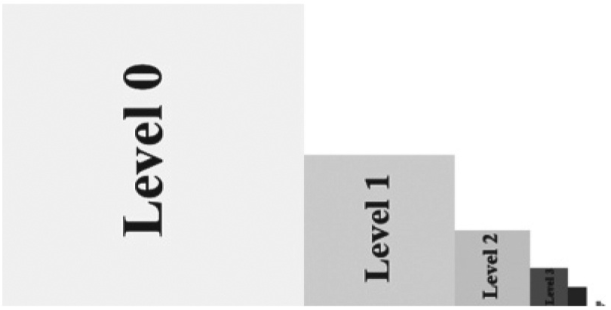
\includegraphics[width=\textwidth]{9-17}
    \centering
    \caption{手动构建的mipmap链,以便每个级别都可以轻松区分。}
\end{figure}

\begin{flushleft}
3.给定两个相同大小的纹理,我们可以通过不同的操作将它们组合起来以获得新的图像。 更一般地,这被称为多纹理,其中使用多个纹理来实现结果。 例如,我们可以添加,减去或(分量)乘以两个纹理的相应纹素。 图\ref{fig:9-18}显示了分量乘以两个纹理以获得类似火球的结果。 在本练习中,通过在图像着色器中组合图\ref{fig:9-18}中的两个源纹理来修改“条箱”演示,使在每个立方体面上生成火球纹理。 (本练习的图像文件可以从本书的网站下载。)请注意,您必须修改Default.hlsl以支持多个纹理。
\end{flushleft}
\begin{figure}[h]
    \label{fig:9-18}
    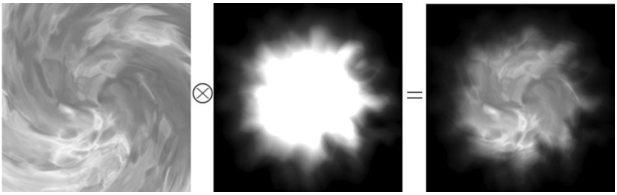
\includegraphics[width=\textwidth]{9-18}
    \centering
    \caption{手动构建的mipmap链,以便每个级别都可以轻松区分。}
\end{figure}

\begin{flushleft}
4.通过在每个立方体面上旋转火球纹理作为时间的函数,将解决方案修改为练习3。\\

5.令$p_{0}$,$p_{1}$和$p_{2}$为具有相应纹理坐标$q_{0}$,$q_{1}$和$q_{2}$的3D三角形的顶点。回想9.2节对于三角形上的任意点$p(s,t)=p_{0}+s(p_{1}-p_{0})+t(p_{2}-p_{0})$其中$s\geq 0$,$t\geq 0$,$s+t\leq 1$,其纹理坐标$(u,v)$是通过相同的$s$,$t$参数在3D三角形上线性插值顶点纹理坐标而得到的:\\
\end{flushleft}
\begin{align*}
(u,v)=q_{0}+s(q_{1}-q_{0})+t(q_{2]-q_{0})
\end{align*}

\begin{itemize}
  \item a.给定$(u,v)$和$q_{0}$,$q_{1}$和$q_{2}$,用$u$和$v$求解$(s,t)$(提示:考虑向量方程$(u,v)=q_{0}+s(q_{1}-q_{0})+t(q_{2}-q_{0})$。
  \item b.表达$p$作为$u$和$v$的函数; 也就是说,找到一个公式$p=p(u,v)$。
  \item c.计算$\partial p/\partial u$和$\partial p/\partial v$并给出这些向量的含义的几何解释。
\end{itemize}

\begin{flushleft}
6.通过向地面,列和球体添加纹理来修改上一章中的“LitColumns”演示(图\ref{9-19})。 纹理可以在本章的代码目录中找到。
\end{flushleft}

\begin{figure}[h]
    \label{fig:9-19}
    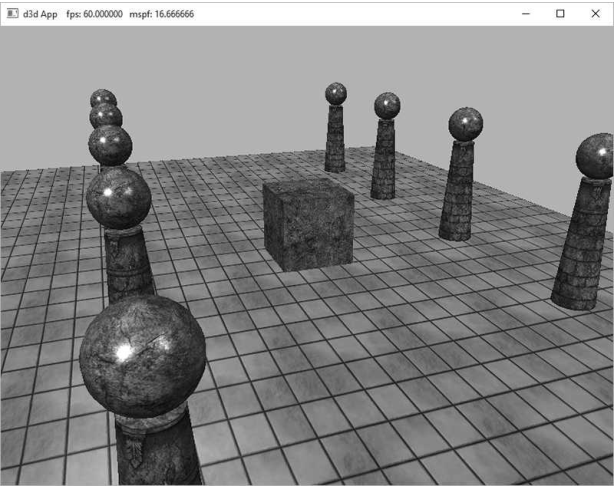
\includegraphics[width=\textwidth]{9-19}
    \centering
    \caption{纹理列场景}
\end{figure}
